\documentclass[aspectratio=169]{beamer}
\usepackage[utf8]{inputenc}
\usepackage{booktabs}
\usepackage{adjustbox}
\usepackage{amsmath,amssymb,amsthm}

\usetheme{Madrid}

\definecolor{mycolor}{rgb}{0.5, 0.5, 0.75}
\definecolor{green}{rgb}{0.3, 0.7, 0.3}
\definecolor{grey}{rgb}{0.4, 0.4, 0.4}
\usecolortheme[named=mycolor]{structure}

\useoutertheme{infolines} % Alternatively: miniframes, infolines, split

\setbeamercolor{palette primary}{bg=green,fg=white} % Titulo, derecha
\setbeamercolor{palette secondary}{bg=green,fg=white} % Medio
\setbeamercolor{palette tertiary}{bg=green,fg=white} % Izquierda
\setbeamercolor{structure}{fg=grey} % Fondos y secciones

\title{Optimal transport for Topological Data Analysis}
\subtitle{Final course thesis}
\author{Gonzalo Ortega}
\date{Wednesday $22^{\text{nd}}$ 2025}

\newcommand{\brc}{\operatorname{Bar}}
\newcommand{\dgmp}{\operatorname{Dgm}_p}
\newcommand{\dgmi}{\operatorname{Dgm}_\infty}

\newcommand{\costp}{\operatorname{cost}_p}
\newcommand{\costi}{\operatorname{cost}_\infty}
\newcommand{\wdp}{\omega_p}
\newcommand{\wdi}{\omega_\infty}
\newcommand{\twdp}{\tilde \omega_p}
\newcommand{\twdi}{\tilde \omega_\infty}
\newcommand{\p}{\mathcal P}
\newcommand{\B}{\brc}
\newcommand{\T}{T_\#}
\newcommand{\N}{\mathbb N}
\newcommand{\R}{\mathbb R}
\newcommand{\upr}{\mathbb{R}_<^2}

\begin{document}

\frame{\titlepage}

\AtBeginSection[]
{
  \begin{frame}{Contents}
    \tableofcontents[currentsection]
  \end{frame}
}

\section{Optimal transport}
\subsection{Preliminaries}
  \begin{frame}
    \frametitle{Preliminaries}
    \framesubtitle{Basic definitions}
    \begin{definition}[Push-forward measure]
      Let $ T: X \to Y $ be a Borel map, and $ \mu \in \p(X)$. Let $ A \in \B $. The {\it push-forward measure} $ \T\mu \in \p(Y) $ is defined as
      $$
          \T\mu(A) := \mu (T^{-1}(A)).
      $$
    \end{definition}

    \begin{definition}[Transport map]
        Given $ \mu \in \p(X) $ and $ \nu \in \p(Y) $, a {\it transport map from $\mu$ to $\nu$} is a Borel map $ T: X \to Y $ that satisfies $ \T\mu = \nu$.
    \end{definition}
  \end{frame}

  \begin{frame}
    \frametitle{Preliminaries}
    \framesubtitle{Basic definitions}
    \begin{definition}[Transport plan]
      Let $\pi_X : (X \times Y) \to X $ and $\pi_Y : (X \times Y) \to Y$ such that for every $(x, y) \in (X, Y) $, $\pi_X(x, y) = x$ and $ \pi_Y(x, y) = y $. A {\it transport plan between $\mu$ and $\nu$} is a probability measure $ \gamma \in \p(X \times Y) $ where
      $$
          (\pi_X)_\# \gamma = \mu \text{ and } (\pi_Y)_\# \gamma = \nu.
      $$
      The set of all couplings between $ \mu $ and $\nu$ is denoted $\Gamma(\mu, \nu)$.
    \end{definition}
  \end{frame}

  \begin{frame}
    \frametitle{Preliminaries}
    \framesubtitle{Monge and Kantorovich formulations}
    \begin{definition}[Transport problems]
      Fix $ \mu \in \p(X)$, $\nu \in \p(Y)$ and consider a lower semicontinous map $ c: X \times Y \to [0, \infty] $. Then
      \begin{align*}
        C_M(\mu, \nu) &:= \inf \left\{\int_X c(x, T(x)) d\mu(x) : \T\mu = \nu \right\}, \\
        C_K(\mu, \nu) &:= \inf \left\{\int_{X \times Y} c(x, y) d\gamma(x,y) : \gamma \in \Gamma(\mu, \nu) \ \right\}.
      \end{align*}
    \end{definition}
  \end{frame}

\subsection{Wasserstein distance over probability spaces}
  \begin{frame}
    \frametitle{Wasserstein distance over probability spaces}
    \begin{definition}[Probability measures with finite $p$-moment]
      Let $ (X, d) $ be a locally compact and separable, metric space. Let $ 1 \leq p < \infty $. The {\it set of probability measures with finite $p$-moment} is defined As
      $$
          \p_p (X) := \left\{ \sigma \in \p (X) : \int_X d(x, x_0)^p d \mu (x) < \infty \text{ for some } x_0 \in X \right\}.
      $$
    \end{definition}

    \begin{definition}[$p$-Wasserstein distance]
      Given $ u, v \in \p_p (X) $, the {\it $p$-Wasserstein distance} is defined as
      $$
          W_p(u, v) := \left( \inf_{\gamma \in \Gamma(u, v)} \int_{X \times X} d(x,y)^p d\gamma(x, y)\right)^{\frac{1}{p}}.
      $$
    \end{definition}
  \end{frame}

\section{Reformulations for TDA}

\subsection{Wasserstein distance over persistence diagrams}
  \begin{frame}
    \frametitle{Wasserstein distance over persistence diagrams}
    \framesubtitle{Basic definitions}
    \begin{definition}[Persistence diagram]
      Let $ I $ be a countable set. A {\it persistence diagram} is a function $ D: I \to \upr $.
    \end{definition}

    \begin{definition}[Partial matching]
      Let $ D_1: I_1 \to \upr $ and $ D_2: I_2 \to \upr $ be persistence diagrams. A {\it partial matching} between $ D_1 $ and $ D_2 $ is the triple $ (I_1', I_2', f) $ such that $ f: I_1' \to I_2' $ is a bijection with $ I_1' \subseteq I_1 $ and $ I_2' \subseteq I_2 $.
    \end{definition}
  \end{frame}

  \begin{frame}
    \frametitle{Wasserstein distance over persistence diagrams}
    \framesubtitle{Tiny diagrams matching example}
    \begin{figure}
      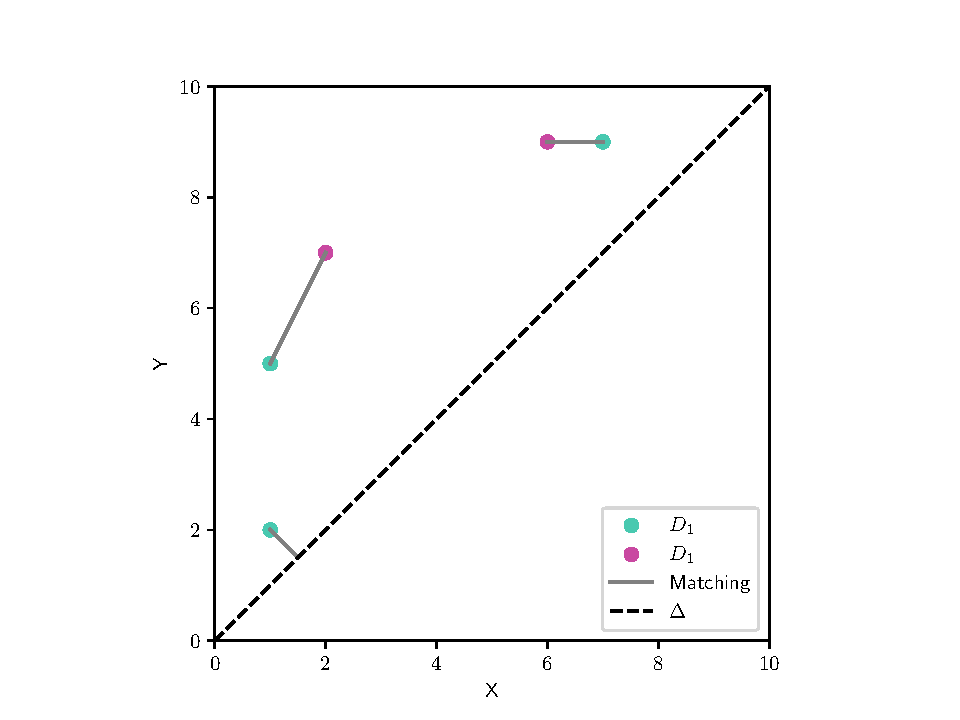
\includegraphics[width=8cm]{../Figures/figure-1.pdf}
    \end{figure}
  \end{frame}

  \begin{frame}
    \frametitle{Wasserstein distance over persistence diagrams}
    \framesubtitle{Chebyshev distance}
    \begin{definition}[Chebyshev distance]
      Let $ a, b \in \R^2 $ with $a = (a_x, a_y) $ and $ b = (b_x, b_y) $. The {\it Chebyshev distance} is defined as
      $$
          d_\infty(a, b) := ||a-b||_{\infty} := \max \{|a_x - b_x|, |a_y - b_y|\}.
      $$
    \end{definition}
  \end{frame}
  
  \begin{frame}
    \frametitle{Wasserstein distance over persistence diagrams}
    \framesubtitle{The cost of a matching}
    \begin{definition}[$p$-cost] \label{def:pcost}
      Let $ D_1: I_1 \to \upr $ and $ D_2: I_2 \to \upr $ be persistence diagrams. Let $ (I_1', I_2', f) $ be a partial matching between them. If $ p < \infty $, the {\it $p$-cost of $ f $} is defined as
      \begin{align*}
          \costp(f) := \bigg(&\sum_{i \in I_1'} d_\infty(D_1(i), D_2(f(i)))^p 
          + \sum_{i \in I_1 \setminus I_1'} d_\infty(D_1(i), \Delta)^p 
          + \sum_{i \in I_2 \setminus I_2'} d_\infty(D_2(i), \Delta)^p \bigg)^{\frac{1}{p}}.
      \end{align*}
      For $ p = \infty $, the {\it $\infty$-cost of $ f $} is defined as
      \begin{align*}
          \costi(f) := \max \bigg\{&\sup_{i \in I_1'} d_\infty(D_1(i), D_2(f_i)), 
          \sup_{i\in I_1 \setminus I_1'} d_\infty(D_1(i), \Delta), 
          \sup_{i\in I_2 \setminus I_2'} d_\infty(D_2(i), \Delta)\bigg\}.
      \end{align*}
    \end{definition}
  \end{frame}

  \begin{frame}
    \frametitle{Wasserstein distance over persistence diagrams}
    \framesubtitle{Bottleneck distance}
    \begin{definition}[p-Wasserstein distance] \label{def:Wasserstein}
      Let $ D_1, D_2 $ be persistence diagrams. Let $ 1 \leq p \leq \infty $. Define
      $$
          \twdp (D_1, D_2) = \inf \{\costp(f) : f \text{ is a partial matching between } D_1 \text{ and } D_2 \}.
      $$
      Let $ \emptyset $ denote the unique persistence diagram with empty indexing set. Let $ (\dgmp, \wdp) $ be the space of persistence diagrams $ D $ that satisfy $ \twdp(D, \emptyset) < \infty $ modulo the equivalence relation $ D_1 \sim D_2 $ if $ \twdp (D_1, D_2) = 0 $. The metric $ \wdp $ is called the {\it $p$-Wasserstein distance}.
    \end{definition}

    \begin{definition}[Bottleneck distance]
      If $ p = \infty $, the metric $ \wdi $ is called the {\it bottleneck distance}.
    \end{definition}
  \end{frame}

\subsection{Metric spaces into persistence diagrams}
  \begin{frame}
    \frametitle{Metric spaces into persistence diagrams}
    \framesubtitle{Definitions}
    \begin{definition}[Isometric embedding]
      Let $ (X, d_X), (Y, d_Y) $ be metric spaces. An {\it isometric embedding} $ \eta: (X, d_X) \to (Y, d_Y) $ is a mapping that satisfies
      $$
          d_X(x_1, x_2) = d_Y(\eta(x_1), \eta(x_2))
      $$
      for all $x_1, x_2 \in X$.
    \end{definition}

    \begin{definition}[Ball in persistence diagrams]
        Let $ 1\leq p \leq \infty $. Let $ D_0 \in \dgmp $. The {\it ball} at the space of persistence diagrams is defined as $ B_p(D_0, r) := \{D \in \dgmp : w_p(D, D_0) < r \} $.
    \end{definition}
  \end{frame}

  \begin{frame}
    \frametitle{Metric spaces into persistence diagrams}
    \framesubtitle{Isometric embeeding}
    \begin{theorem}[Isometric embeeding of metric spaces into persistance diagrams]
      Let $ (X, d) $ be a separable, bounded metric space. Then there exists an isometric embedding to the space of persistence diagrams $ \eta: (X, d) \to (\dgmi, \wdi)$ such that $ \eta(X) \subseteq B(\emptyset, \frac{3c}{c}) \backslash B(\emptyset, c) $.
    \end{theorem}
  \end{frame}
  \begin{frame}
    \frametitle{Metric spaces into persistence diagrams}
    \framesubtitle{An example}
    As $ (X, d) $ is bounded, we can let $ c > \sup \{d(x, y): \  x, y \in X\} $. As $ (X, d) $ is separable, we can take $ \{x_k\}_{k=1}^\infty $, a countable, dense subset of $ (X, d) $. Consider
      \begin{align*}
          \eta: (X, d) &\to (\dgmi, \wdi) \\
          x &\mapsto \{(2c(k-1), 2ck + d(x, x_k))\}_{k=1}^\infty
      \end{align*}
    \begin{figure}
      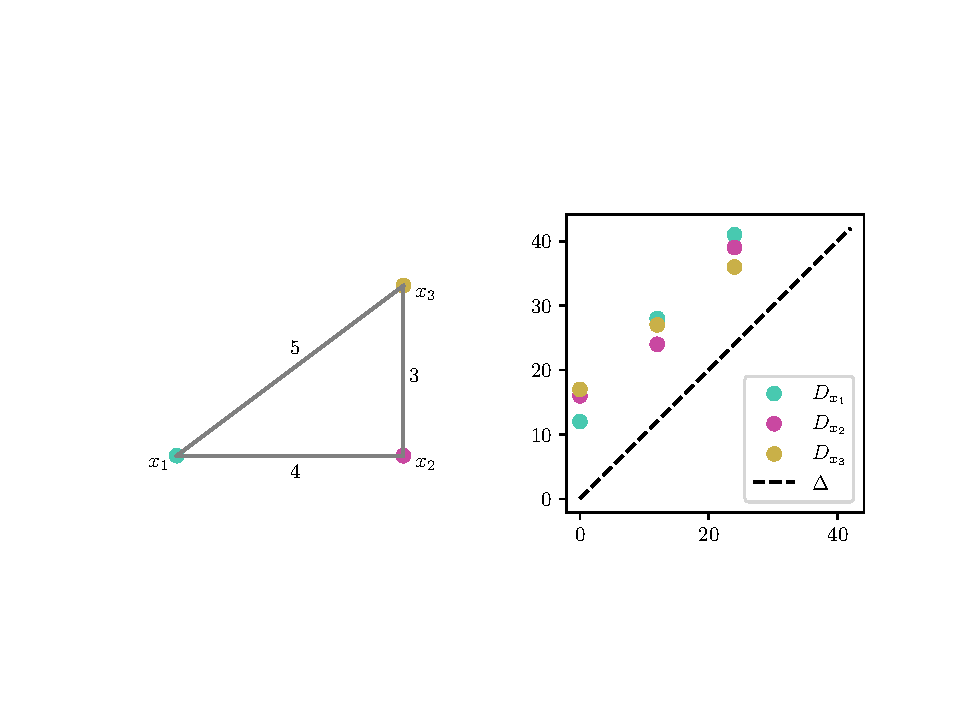
\includegraphics[trim={0 0 0 3cm},clip, width=10cm]{../Figures/figure-2.pdf}
    \end{figure}
  \end{frame}

\end{document}
